\documentclass[tikz]{standalone}
\usepackage{tikz}
\usetikzlibrary{decorations.markings}

\begin{document}

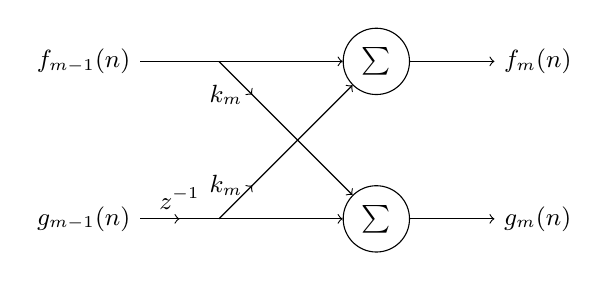
\begin{tikzpicture}[font=\small]
    \tikzset{
        zdelay/.style={
            postaction={decorate},
            decoration={
                markings,
                mark=at position 0.5 with {
                    \arrow{>};
                    \node[above]{$z^{-1}$};
                }
            }
        },
        kgain/.style={
            postaction={decorate},
            decoration={
                markings,
                mark=at position 0.25 with {
                    \arrow{>};
                    \node[left]{#1};
                }
            }
        }
    }

    \coordinate (f0c) at (0,0);
    \coordinate (g0c) at ([yshift=-2cm] f0c);
    \node (f0) at ([xshift=-1cm] f0c) [left]{$f_{m-1}(n)$};
    \node (g0) at ([xshift=-1cm] g0c) [left]{$g_{m-1}(n)$};
    \node[circle,draw] (sf1) at ([xshift=2cm] f0c) {$\sum$};
    \node[circle,draw] (sg1) at ([xshift=2cm] g0c) {$\sum$};
    \node (f1) at ([xshift=3.5cm] f0c) [right]{$f_m(n)$};
    \node (g1) at ([xshift=3.5cm] g0c) [right]{$g_m(n)$};

    \draw (f0) -- (f0c);
    \draw[zdelay] (g0) -- (g0c);
    \draw[->] (f0c) -- (sf1);
    \draw[->] (g0c) -- (sg1);
    \draw[->,kgain={$k_m$}] (f0c) -- (sg1);
    \draw[->,kgain={$k_m$}] (g0c) -- (sf1);
    \draw[->] (sf1) -- (f1);
    \draw[->] (sg1) -- (g1);
\end{tikzpicture}

\end{document}